\newpage
\section{Conclusiones}
\label{conclusiones}

A lo largo de nuestra tesis se han investigado numerosas herramientas de
\eng{software} para construir una solución de monitoreo para el
\gls{acro:cespi}.

En primer lugar se ha configurado \gls{term:influx} para almacenar métricas de
tipo series de tiempo. Se ha mostrado cómo hacer para que las aplicaciones
\gls{term:ror} sean ejecutadas dentro de \glspl{term:contenedor} de
\gls{term:docker} y cómo lograr que envíen información a \gls{term:influx} a
través de la \gls{term:gema} \texttt{influxdb-rails}.

\begin{figure}
  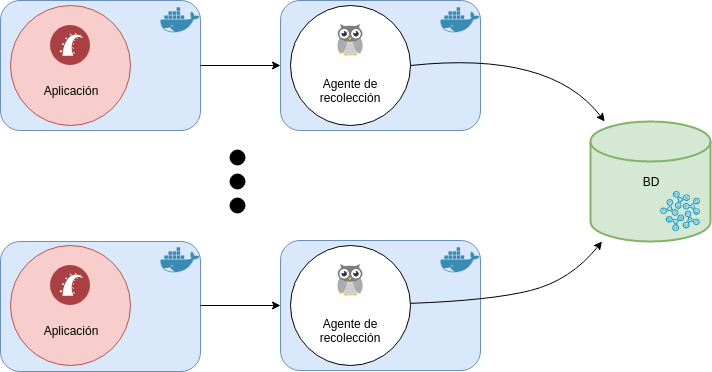
\includegraphics[width=\linewidth]{src/images/conclusiones/influx.png}
  \caption{\gls{term:cadvisor} toma información de los contenedores de las
    aplicaciones y se la envía a \gls{term:influx}}
  \label{fig:diagrama-influx}
\end{figure}

Además se ha mostrado cómo configurar \gls{term:cadvisor} para
obtener valiosa información del sistema y enviarla a \gls{term:influx}.
(\autoref{fig:diagrama-influx})

\begin{figure}
  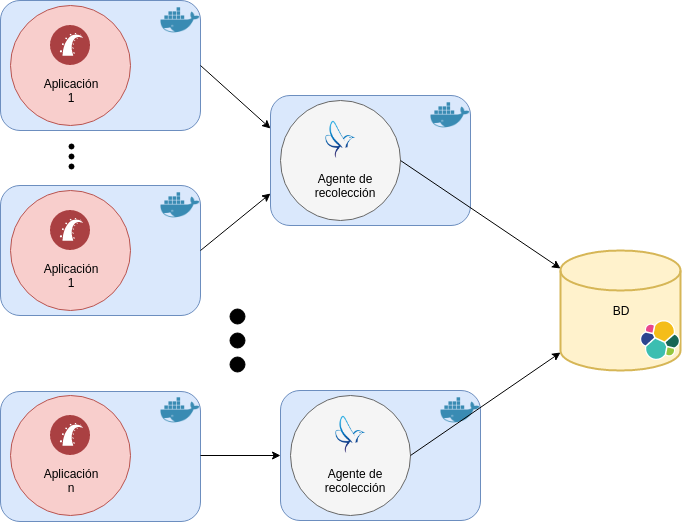
\includegraphics[width=\linewidth]{src/images/conclusiones/elastic.png}
  \caption{\gls{term:fluentd} recolecta los logs de las
    aplicaciones y se las envía a \gls{term:elasticsearch}}
  \label{fig:diagrama-elastic}
\end{figure}

También se ha descripto cómo configurar \gls{term:nginx} y las aplicaciones
para recuperar los datos de sus \eng{logs} e imprimirlos en el \gls{acro:stdout}
del \gls{term:contenedor} de \gls{term:docker} para luego enviarlos a
través de \gls{term:fluentd} a \gls{term:elasticsearch}. De esta forma se ha
logrado utilizar toda la información guardada en \eng{logs} que antes era
desaprovechada. (\autoref{fig:diagrama-elastic})

Se ha demostrado cómo usar \gls{term:kibana} para crear gráficos a partir de la
información de los \eng{logs} en \gls{term:elasticsearch} y realizar la exploración
de los \eng{logs} de forma sencilla, y cómo configurar un tablero de
\gls{term:grafana} para mostrar los datos almacenados en \gls{term:influx}.

\begin{figure}
  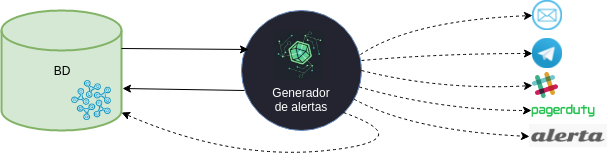
\includegraphics[width=\linewidth]{src/images/conclusiones/alerts.png}
  \caption{\gls{term:kapacitor} genera alertas a diferentes destinos a partir
    de información tomada de \gls{term:influx}}
  \label{fig:diagrama-alerts}
\end{figure}

Finalmente se ha configurado \gls{term:kapacitor} para generar alertas útiles,
definiendolas en el lenguaje \gls{term:tick_script} y luego se ha usado la
herramienta \gls{term:alerta} para resolver el problema de múltiples alertas.
(\autoref{fig:diagrama-alerts})

Durante el transcurso de la investigación se han explorado otras
herramientas como \gls{term:logstash}, \gls{term:opentsdb}, \gls{term:graphite}
y \gls{term:telegraf}, que finalmente no formaron parte de la solución.

Ninguna herramienta cumplía con todas las características que la solución
propuesta demandaba, por lo que muchas veces se ha resuelto sólo tomar parte de
las funcionalidades de cada herramienta para resolver el problema.

Se ha logrado construir una solución de monitoreo que se acopla al diseño de la
infraestructura, y se ha hecho utilizando solamente herramientas gratuitas,
de código abierto y albergadas por la misma oficina (\eng{self-hosted}).

El sistema que se ha diseñado puede utilizarse para armar tableros y alertas
que permitan mejorar el proceso de toma de decisiones para todos los roles de
la organización.

Se ha construido una solución de monitoreo base para que el
área de desarrollo del \gls{acro:cespi} pueda realizar un control básico y
efectivo de sus aplicaciones, y la extienda de acuerdo a los atributos que crea
necesario medir en cada aplicación.

Esta solución se ajusta perfectamente a la escalabilidad, dinamismo
y automatización con los que cuenta la infraestructura.

El monitoreo es una rama de investigación que sigue creciendo cada día. Si bien
actualmente existen varias herramientas relacionadas con el monitoreo, creemos
que en un futuro se contará con herramientas más completas.

Durante el desarrollo de la tesis se ha tenido que investigar sobre disciplinas
ajenas a la informática, como lo son la administración de proyectos, la
estadística, la visualización efectiva de información e incluso la psicología.

Hemos aprendido acerca de la importancia del monitoreo para resolver problemas
rápidamente, estudiar el comportamiento de los sistemas y aplicaciones y tomar
decisiones para mejorar la implementación de los procesos de desarrollo, la
infraestructura de \eng{software} y las aplicaciones.
